\documentclass[11pt]{article}
\usepackage{amsmath,amssymb,graphicx,xcolor,tikz}
\usetikzlibrary{arrows.meta,calc,positioning}
\newcommand{\M}{\mathcal M}
\newcommand{\R}{\mathbb R}
\newcommand{\T}{\mathsf T}
\newcommand{\Wwin}{\mathcal W}
\newcommand{\Hscore}{\mathcal H}
\DeclareMathOperator{\reach}{reach}
% Numbering in the submitted manuscript.
\makeatletter
\newlabel{prop:pilot}{{3.1}{}}
\newlabel{prop:step}{{3.2}{}}
\newlabel{prop:finite}{{3.3}{}}
\newlabel{prop:readout}{{3.4}{}}
\newlabel{thm:isolated-rank}{{3.5}{}}
\makeatother
\pagestyle{empty}
\begin{document}
\setbox0=\hbox\bgroup
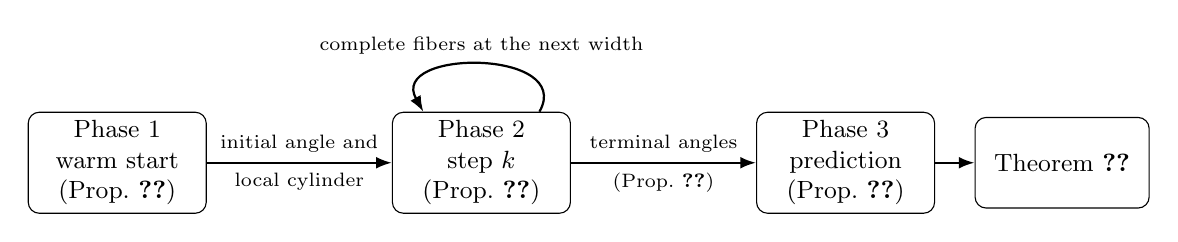
\begin{tikzpicture}[
  box/.style={draw, rounded corners, align=center, inner sep=3pt, font=\small,
              minimum height=1.15cm, text width=2.05cm},
  lab/.style={font=\scriptsize, align=center},
  arr/.style={-{Latex[length=2mm]}, thick}]
\node[box] (p1) {Phase 1\\warm start\\(Prop.~\ref{prop:pilot})};
\node[box, right=2.35cm of p1] (p2) {Phase 2\\step $k$\\(Prop.~\ref{prop:step})};
\node[box, right=2.35cm of p2] (p3) {Phase 3\\prediction\\(Prop.~\ref{prop:readout})};
\node[box, text width=2.0cm, right=0.5cm of p3] (th) {Theorem~\ref{thm:isolated-rank}};
\draw[arr] (p1) -- node[lab, above] {initial angle and} node[lab, below] {local cylinder} (p2);
\draw[arr] ([xshift=-4mm]p2.north east) .. controls +(0.45,0.8) and +(-0.45,0.8) .. ([xshift=4mm]p2.north west)
  node[lab, pos=0.5, above] {complete fibers at the next width};
\draw[arr] (p2) -- node[lab, above] {terminal angles} node[lab, below] {(Prop.~\ref{prop:finite})} (p3);
\draw[arr] (p3) -- (th);
\end{tikzpicture}
\egroup
\pdfpagewidth=\dimexpr\wd0+4pt\relax
\pdfpageheight=\dimexpr\ht0+\dp0+4pt\relax
\hoffset=-1in \voffset=-1in
\shipout\vbox{\kern2pt\hbox{\kern2pt\box0}}
\end{document}
